\documentclass{article}[18pt]
\usepackage{../../../../../format}
\lhead{MCS - DMLA}


\begin{document}
\begin{center}
\underline{\huge Paths, Cycles and Connectivity}
\end{center}
\section{Walks, paths, cycles and distances}
\begin{itemize}
	\item A walk in a graph G is a sequence $v_0v_1,v_1,v_2,...,v_{n-1}v_n$. In this case we also say that $v_0,v_1,...v_n$ is a walk of G
	\item A walk $v_0,v_1,...,v_n$ in G is a path is all $v_i$'s are distinct. In this case we also say that $v_0,v_1,...,v_n$ is a graph in G. A \textbf{path} is a walk that never crosses itself
	\item A walk $v_0,v_1,...,v_n$ with $v_0=v_n$ is called a \textbf{circuit} or \textbf{closed walk}
	\item A closed walk is a \textbf{cycle} if all $v_i$'s in it are distinct except $v_0=v_n$
	\item If G is a directed graph then the \textbf{directed paths} and \textbf{directed cycles} are defined in a natural way, with each edge being directed from $v_i$ to $v_{i+1}$
	\item The \textbf{length} of a path or a cycle is the number of edges in it
	\item The distance between vertices u and v in a graph, denotes $dist(u,v)$, is the length of a shortest path from u to v if such a path exists, and $\infty$ otherwise
	\item The \textbf{diameter} of a graph is the largest distance between two vertices in it
\end{itemize}
\section{The acquaintance graph and six degrees of separation}
\begin{itemize}
	\item All vertices are people
	\item There is an edge between two of them if they are acquainted
\end{itemize}
\section{The collaboration graph and the Erdos number}
\begin{itemize}
	\item The vertices are all people
	\item There is an edge between two of then if they have written a joint paper
\end{itemize}
\section{Shortest Path Problems}
In an edge weighted graph, the problem of finding the shortest distance from u to v is the shortest path problem

\section{Connectivity}
\subsection{Definition}
A graph is called \textbf{connected} if any two distinct vertices are connected by a path. A \textbf{connected component} of a graph G is a maximal connected subgraph of G
\begin{center}
	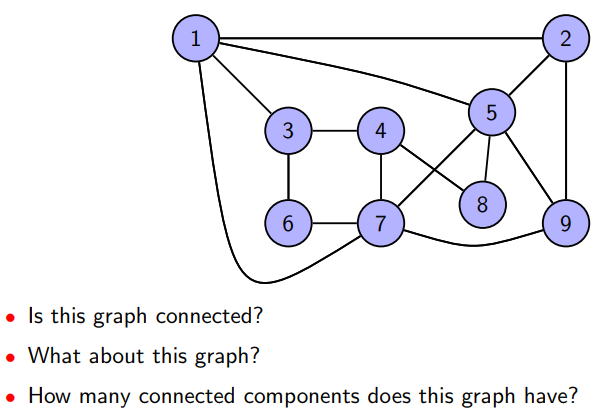
\includegraphics[scale=0.7]{grapj}
\end{center}
\begin{itemize}
	\item Is connected - In one piece 
	\item Removing 6-7, 5-8 and 4-7 makes two connected components, making it not connected
\end{itemize}
\section{Exercise}
$\delta$  - the smallest degree of a vertex in a graph\\
\\
Prove that if G is a graph on n vertices are $\delta(G)\geqslant (n-1)/2$ then G is connected
\begin{itemize}
	\item Proof \textbf{by contradiction:} Assume G is not connected, derive a contradiction
	\item Take two vertices u and v in different connected components
	\item We have that $deg(u)\geqslant (n-1)/2$ and $deg(v)\geqslant (n-1)/2$
	\item The set N(u) contains none of the neighbours of v nor v itself
	\item Similarly, N(v)  contains none of the neighbours of u nor u itself
	\item Hence G contains at least $\frac { n - 1 } { 2 } + 1 + \frac { n - 1 } { 2 } + 1 = n + 1$ vertices, a contradiction
	\item In fact, we even proved more: any two vertices in G are at distance at most 2 (so the diameter of G is at most 2)
\end{itemize}
\section{Strong connectivity}
\subsection{Definition}
\begin{itemize}
	\item A directed graph G is called \textbf{(weakly) connected} if the graph obtained from G by forgetting directions is connected
	\item A directed graph is called \textbf{strongly connected} if any two distinct vertices are connected by directed paths in both directions (can go from u to v and v to u)
	\item A \textbf{strongly connected component} (or simply \textbf{strong component}) of a digraph G is a maximal strongly connected subgraph of G
\end{itemize}
Graph
\begin{itemize}
	\item 3,4,6,7 is a strongly connected component as a loop is formed, the only way out is to go to 8, which you cannot leave
	\item 2,1,5,9 is another strongly connected component
	\item 8 is a strong component on its own
\end{itemize}
\section{Special circuits/cycles in graphs}
\begin{itemize}
	\item Can we travel along the edges of a given graph G so that we start and finish at the same verted and traverse \textbf{each edge exactly once}?
	\begin{itemize}
		\item Such a circuit in G is called a Eulerian circuit
	\end{itemize}
	\item Can we travel along the edges of a given graph so that we start and finish at the same vertex and visit \textbf{each vertex exactly once}
	\begin{itemize}
		\item Such a called a \textbf{Hamiltonian} cycle
	\end{itemize}
\end{itemize}



\end{document}